\chapter{KIẾN TRÚC HỆ THỐNG}
\label{chapter3}
Từ những cơ sở lý thuyết thu thập ở chương 2, chương này em sẽ trình bày những bước giải quyết bài toán mà đề tài đưa ra.
\section{Phân tích yêu cầu}
Từ yêu cầu của đề tài và việc phân tích chi tiết yêu cầu và chức năng của hệ thống cần phải đáp ứng, em đã xác định được yêu cầu chức năng và phi chức năng của hệ thống như sau:
\begin{itemize}
\item	Yêu cầu chức năng:
	\begin{itemize}
	\item	Các nút truyền dữ liệu đến được Gateway,
	\item	Mạng có linh động về số lượng nút,
	\item	Số lượng nút trong mạng từ 3 nút trở lên.
	\end{itemize}
\item Yêu cầu phi chức năng:  
	\begin{itemize}
	\item 	Các nút truyền dữ liệu chính xác, ổn định,
	\item 	Nút tiêu tốn ít năng lượng,
	\item	Thiết bị hoạt động ổn định,
	\item	Hình thức gọn, phù hợp điều kiện làm việc.
	\item	Dữ liệu được đảm bảo an toàn,
	\item	Chi phí hợp lý.
	\end{itemize}
\end{itemize}
\section{Kiến trúc tổng thể hệ thống}
Dựa trên cơ sở kiến trúc đã có sẵn của thiết bị BKRES, hệ thống sẽ được tích hợp thêm module truyền thông LoRa vào các thiết bị của hệ thống. Khi đó hệ thống gồm 4 phân hệ chính. Hình \ref{construction}{} mô tỏ rõ hơn kiến trúc hệ thống.
\begin{itemize}
	\item Phân hệ cảm biến và xử lý dữ liệu: Ở mỗi nút mạng được trang bị các bộ cảm biến ghi đo 4 tham số (hàm lượng Oxy, nhiệt độ, độ pH và nồng độ muối). Dữ liệu cảm biến được gửi đến bộ điều khiển trung tâm (sử dụng vi điều khiển STM32) để xử lý, phân tích, đóng gói và gửi đến module truyền thông LoRa.
	\item Phân hệ truyền thông sử dụng LoRa: hoạt động theo mô hình đơn chặng, có nhiệm vụ gửi dữ liệu từ phân hệ cảm biến tới server trung tâm.
	\item Phân hệ cung cấp dịch vụ: Sau khi nhận dữ liệu từ phân hệ truyền thông, phân hệ này có nhiệm vụ xử lý dữ liệu và cung cấp các dịch vụ cho phân hệ giám sát và người dùng.
	\item Phân hệ giám sát và điều khiển: có nhiệm vụ hiển thị dữ liệu cảm biến một cách trực quan thông qua ứng dụng di động, ứng dụng web. Người dùng có thể cấu hình hệ thống, đặt các mức ngưỡng cảnh báo,… trên ứng dụng.
\end{itemize}
\begin{center}
\begin{figure}
\begin{center}
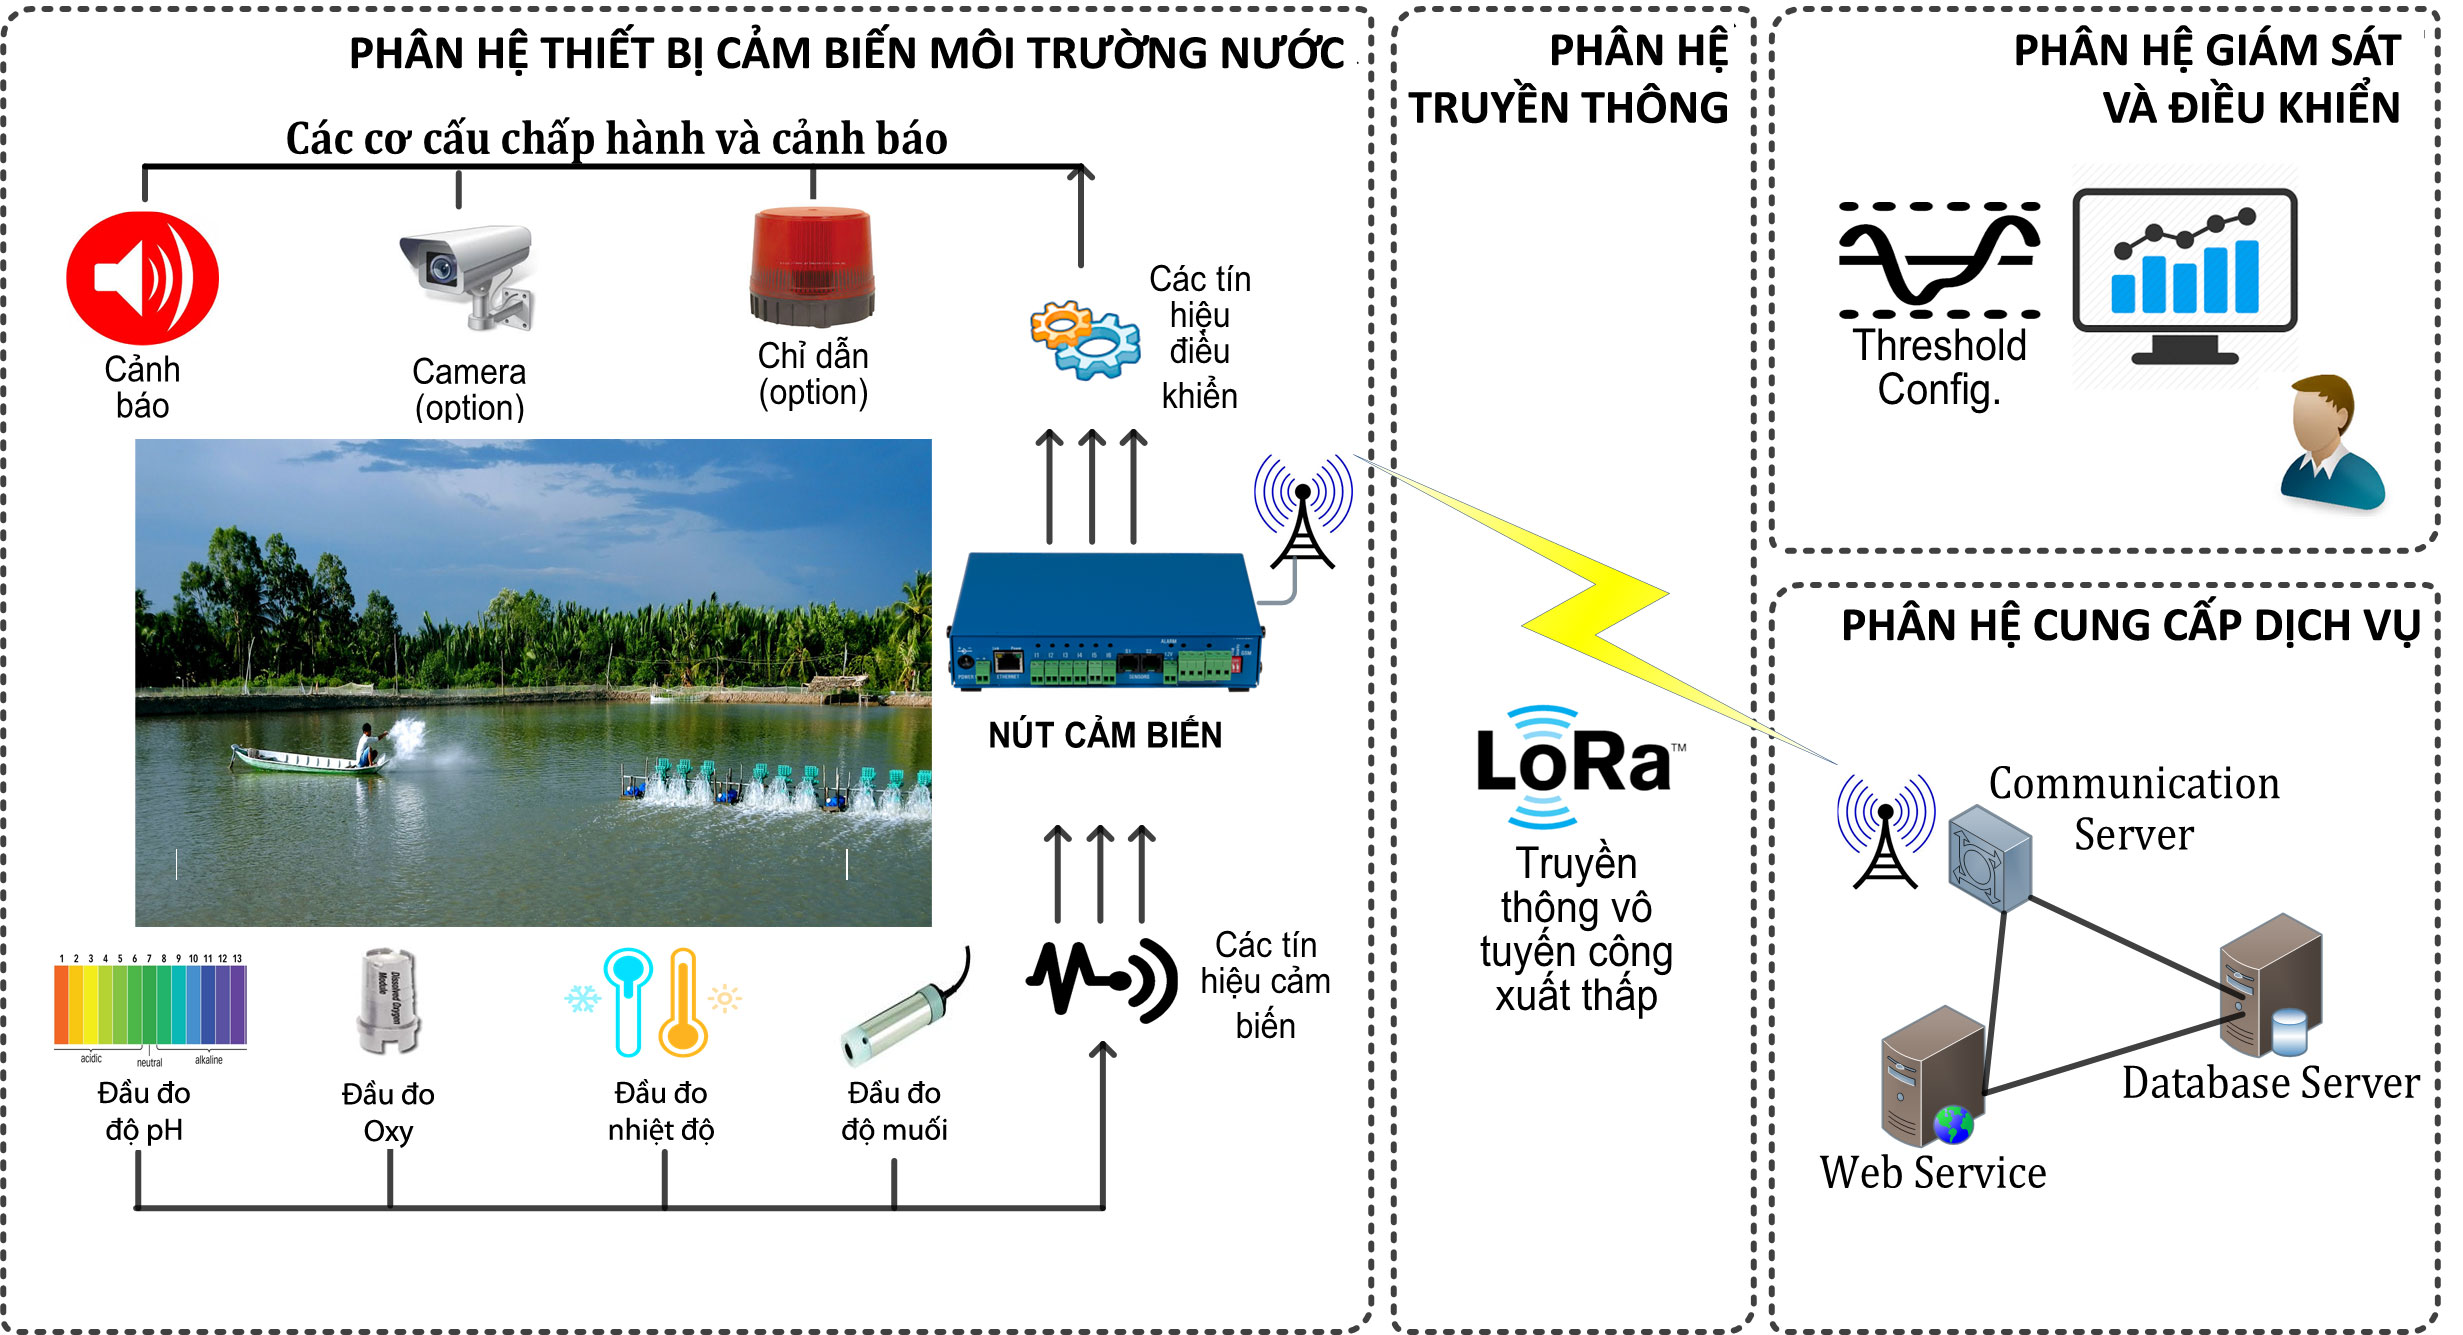
\includegraphics[scale=0.15]{image/kientrucLoRa}
\end{center}
\caption{Kiến trúc hệ thống}
\label{construction}
\end{figure}
\end{center}
\par 
Module LoRa SX1278 được lựa chọn để tích hợp vào thiết bị cảm biến như thể hiện trên hình \ref{moduleSX1278}{}. Nút cảm biến được thiết kế và chế tạo tài phòng nghiên cứu SANSLAB, gồm các thành phần phần cứng chính như: phân hệ cảm biến các tham số môi trường nước, phân hệ truyền thông, phân hệ vi xử lý và điều khiển, phân hệ cấp nguồn và phân hệ hiển thị, cảnh tại chỗ. Phần mềm trên nút cảm biến gồm firmware và drivers điều khiển hoạt động các phân hệ và ngoại vi, thuật toán đa truy nhập cũng được nhúng trong firmware của thiết bị. Một số thuật toán chính được biểu diễn qua các lưu đồ sau đây.
\section{Thiết kế nút mạng cảm biến tích hợp~module SX1278}
%\begin{center}
\begin{figure}[h]
	\begin{center}
		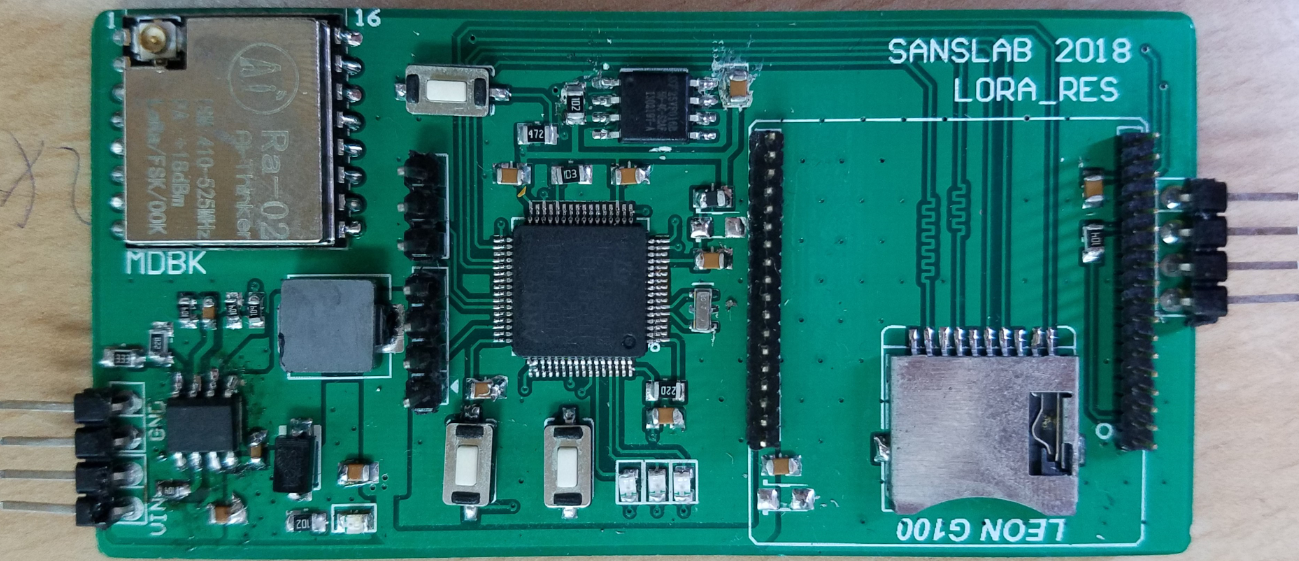
\includegraphics[scale=0.45]{image/hinh3_1}
	\end{center}
	\caption{Nút cảm biến tích hợp chip LoRa SX1278}
	\label{moduleSX1278}
\end{figure}
%\end{center}
\section{Mô hình mạng hình sao}
Thuật toán đa truy nhập đề xuất được phát triển và thử nghiệm trên mô hình gồm 3 nút cảm biến và một Gateway như hình \ref{protocol}{}. Để đánh giá khả năng truyền dữ liệu, độ ổn định, khả năng tùy biến và tự cấu hình của các nút trong mạng, em cấu hình các thông số cơ bản của các nút theo như bảng \ref{bang3_1}{}.
\begin{table}[h]
	\tabcolsep = 2cm
    \centering
    \caption{Bảng thông số cấu hình của các nút trong mạng}
    \begin{tabular}{|c|c|}
     	\hline
     	Thông số & Giá trị  \\
     	\hline
     	Channel & 11 (433 MHz)\\
     	\hline
     	BW & 125 kHz\\
     	\hline
     	CR & 4/5\\
     	\hline
     	SF & 7\\
     	\hline
     	Header & ON\\
     	\hline
     	CRC & ON\\
     	\hline
    \end{tabular}
    \label{bang3_1}
\end{table}
\par 
Khi mô hình hoạt động bình thường (hình \ref{normal}{}), 3 nút sẽ gửi dữ liệu đến Gateway theo một chu kỳ định sẵn. Trong thí nghiệm để kiếm tra sự ổn định của mạng một số thông số khoảng các của các nút với Gateway sẽ được thay đổi.\\
\begin{center}
\begin{figure}[h]
	\begin{center}
		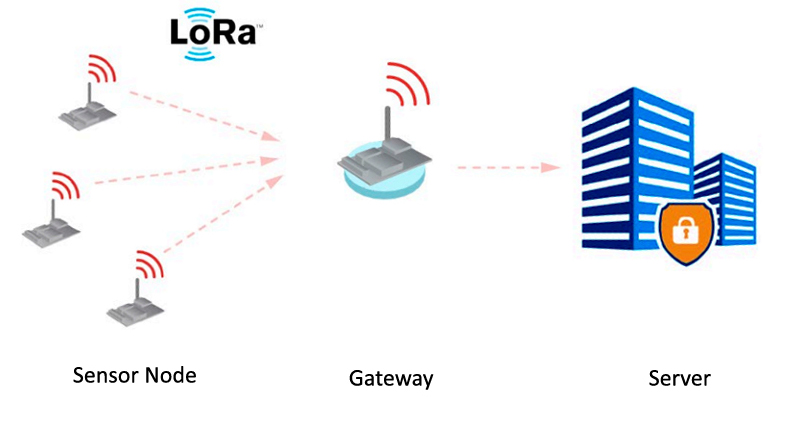
\includegraphics[scale=0.35]{image/normal}
	\end{center}
	\caption{Mô hình hoạt động của mạng}
	\label{normal}
\end{figure}
\end{center}
\par 
Trong trường hợp mạng đang hoạt động bình thường, có một nút mới tham gia vào mạng, nút này sẽ gửi yêu cầu đến Gateway. Sau khi được Gateway chấp nhận thì nút sẽ gửi dữ liệu đến Gateway theo một chu kỳ như những nút khác.
\section{Xây dựng lưu đồ thuật toán xử lý trên STM32}   
Với mô hình truyền thông hình sao như đề xuất trên, module truyền thông SX1278 trên mỗi nút mạng trong hệ thống được điều khiển bởi vi xử lý STM32 thông qua giao tiếp UART. Một số thuật toán điều khiển hoạt động của nút được trình bày trong các phần sau đây. 
\subsection{Gateway} 
 Trong quá trình truyền nhận dữ liệu, Gateway có các chức năng chính sau:
 \begin{itemize}
 \item	Gateway tự động cấu hình,
 \item	Nhận dữ liệu từ các nút,
 \item	Quản lý nút trong mạng.
 \end{itemize}
 \par 
Sau khi đã cấu hình cho gateway, trong vòng lặp vô hạn, gateway liên tục mở kênh truyền để nhận bản tin. Nếu bản tin đó là do một nút mới gửi đến (nút chưa tham gia vào mạng) thì gateway sẽ tiến hành quá trình xác thực nút. Còn nếu bản tin là bản tin chứa dữ liệu, Gateway sẽ nhận và xử lý dữ liệu và tiếp tục quá trình mở kênh truyền để nhận dữ liệu. Thuật toán \ref{gateway} thể hiện thuật toán xử lý của Gateway.
\begin{center}
\begin{algorithm}[h]
	\caption{Thuật toán của Gateway}
	\label{gateway}
	\begin{algorithmic}[1]
		\State $pass \gets sanslab$
		\State Gateway tự động cấu hình  \Comment{Gateway sẽ tự động cài một số thông số như ID, SF, CR, tần số,...}
		\While{1}
			\If{Nhận được gói tin}
				\State $packet \gets packet\_receive$	\Comment{gói tin nhận được}
				\If{$packet$ là gói tin gửi dữ liệu}
					\State $data \gets packet.data$
					\State Xử lý dữ liệu	\Comment{Gateway có thể gửi dữ liệu lên Server, hiển thị hoặc lưu dữ liệu}
				\ElsIf{$packet$ là gói tin yêu cầu tham gia mạng}
					\State	$ID \gets packet.src$	\Comment{Lấy ID của nút gửi đến}
					\State	$authentication \gets packet.data$ \Comment{Lấy dữ liệu bản tin xác thực}
					\State 	$response \gets true$
					\If{$authentication \neq pass$ }
						\State $response \gets flase$
					\EndIf
					\State gửi bản tin phản hồi response cho nút ID
				\EndIf
			\EndIf		
		\EndWhile
	\end{algorithmic}
\end{algorithm}
\end{center}
\subsection{Nút} 
Trong quá trình truyền nhận dữ liệu, nút có các chức năng chính sau:
\begin{itemize}
\item	Nút tự động cấu hình, mỗi nút có một ID khác nhau,
\item	Khi nút chưa tham gia mạng, nút sẽ gửi yêu cầu để tham gia mạng. Khi đó xảy ra một số trường hợp sau:
	\begin{itemize}
	\item	Quá trình yêu cầu không thành công, nút sẽ gửi lại,
	\item	Nếu bản tin xác thực sai, nút sẽ không hoạt động nữa,
	\item	Nếu quá trình yêu cầu tham gia mạng thành công, nút sẽ gửi dữ liệu.
	\end{itemize}
\item	Sau khi tham gia mạng thành công, nút sẽ gửi dữ liệu theo chu kỳ.
\end{itemize}
Sau khi được cấu hình, nút sẽ gửi bản tin xác thực cho Gateway (ID của Gateway được cấu hình sẵn trong nút). Nút sẽ thực hiện quá trình yêu cầu tham gia mạng (\ref{RequestJoinNetworks}) đến khi thành công (nếu bản tin xác thực sai, nút sẽ dừng lại). Sau khi nút nhận được bản tin chấp nhận tham gia vào mạng của Gateway, nút sẽ tiến hành quá trình gửi dữ liệu (quá trình này được thực hiên theo chu kỳ). Quá trình xử lý của nút được thể hiện \ref{node}{}.
\begin{center}
\begin{algorithm}[h]
	\caption{Thuật toán của Nút}
	\label{node}
	\begin{algorithmic}[1]
		\State {$msgAuthentication \gets sanslab$}
		\State Nút tự động cấu hình  \Comment{Nút sẽ tự động cài một số thông số như ID, SF, CR, tần số,...}
		
		\State {$idGateway \gets$ Địa chỉ Gateway}		
		\State {$response \gets 2 $} \Comment{response = 0 --> bản tin xác thực chính xác; response = 1 --> bản tin xác thực không chính xác; response = 2 --> nút chưa tham gia mạng}
		
		\State $RequestJoinNetworks(idGateway, msgAuthentication)$
		
		\While{1}
			\If{$response == 0$}
				\State $data \gets$ lấy dữ liệu từ cảm biến
				\State $cnt = 0$
				\Repeat
					\State $state \gets sendPacket(idGateway, data)$ 
					\If{$state > 0$} 
						\State Delay()
					\EndIf
					\State $cnt \gets cnt + 1$
				\Until{$state > 0$ and $cnt < threshold$} \Comment{threshold là số lần gửi tối đa}
			\ElsIf{$response == 1$} 
				\State $Sleep()$ 
				\Else
					\State $RequestJoinNetworks(idGateway, msgAuthentication)$
				\EndIf
			%\EndIf
		\EndWhile
	\end{algorithmic}
\end{algorithm}
\end{center}
\par 
Trong quá trình yêu cầu tham gia vào mạng, nút sẽ gửi bản tin xác thực đến khi nào nhận lại được bản tin phản hồi của Gateway. Khi đó nút sẽ biết đươc mình đã được chấp thuận tham gia mạng hay chưa. Còn về phần Gateway, sau khi nhận được bản tin xác thực được gửi từ nút, Gateway sẽ kiểm tra bản tin xác thực đó có chính xác không. Kết quả của quá trình kiểm tra bản tin xác thực sẽ được Gateway gửi lại cho nút
\begin{algorithm}
\caption{RequestJoinNetworks}
\label{RequestJoinNetworks}
\begin{algorithmic}[1]
  \Procedure {RequestJoinNetworks}{$idGateway$, $msgAuthentication$}
	\Repeat
			\State $state \gets sendPacket(idGateway, msgAuthentication)$ 
			\Comment{state là trạng thái của quá trình gửi tin; state = 0 gửi bản tin thành công; state > 0 gửi bản tin chưa thành công}
			\If{$state > 0$} 
				\State Delay()
			\ElsIf{Nhận được bản tin hồi đáp từ Gateway}
				\State $response \gets packet\_receive.data$
				\If{$response$ không chính xác} 
					\State $state \gets 1$
				\EndIf
			\EndIf
	\Until{$state > 0$}
  \EndProcedure
\end{algorithmic}
\end{algorithm}
\section{Kết luận}
Trong chương 3, em đã trình bày mô tả giao thức đa truy nhập mà em đã xây dựng để giải quyết đề tài. Sau quá trình xây dựng, triển khai và thí nghiệm, em xin trình bày kết quả đạt được trong chương sau.



